\documentclass[11pt]{article}
\usepackage{graphicx}

\begin{document}
	\begin{center}
		\begin{Large}
			Assignment No 3
		\end{Large}
	\end{center}•
	Aim:Implementation of LALR parser to evaluate given expression using Lex and Yacc.\\
	
	\noindent
	Objective:
	\begin{enumerate}
		\item To understand the basic syntax of YACC specifications, built-in functions and variables.
		\item To understand the construction of LALR Parser.
		\item To design LALR parser to evaluate given expression.
	\end{enumerate}•
	
	\noindent
	Software Requirement:
	\begin{enumerate}
		\item Linux Operating System
		\item Lex compiler
		\item Yacc compiler
	\end{enumerate}•
	
	\noindent
	Mathematical Model:\\
	Consider a set S consisting of all the elements related to a program.The mathematical model is given as below,\\ S={s,e,X,Y,Fme,DD,NDD,Mem shared} Where, s = Initial State e = End State\\
	X = Input data. Here it is Expression.Example of expressions: sum=20,count=10,sum+count Y = Output.Here output is value of the expression.\\
	Fme = Algorithm/Function used in program.for eg.{int insert(char tok[10])}\\
	DD = Deterministic Data\\
	NDD = Non deterministic Data\\
	Mem shared = Memory shared by processor.\\
	
	\noindent
	Theory:\\
	
	\begin{center}
		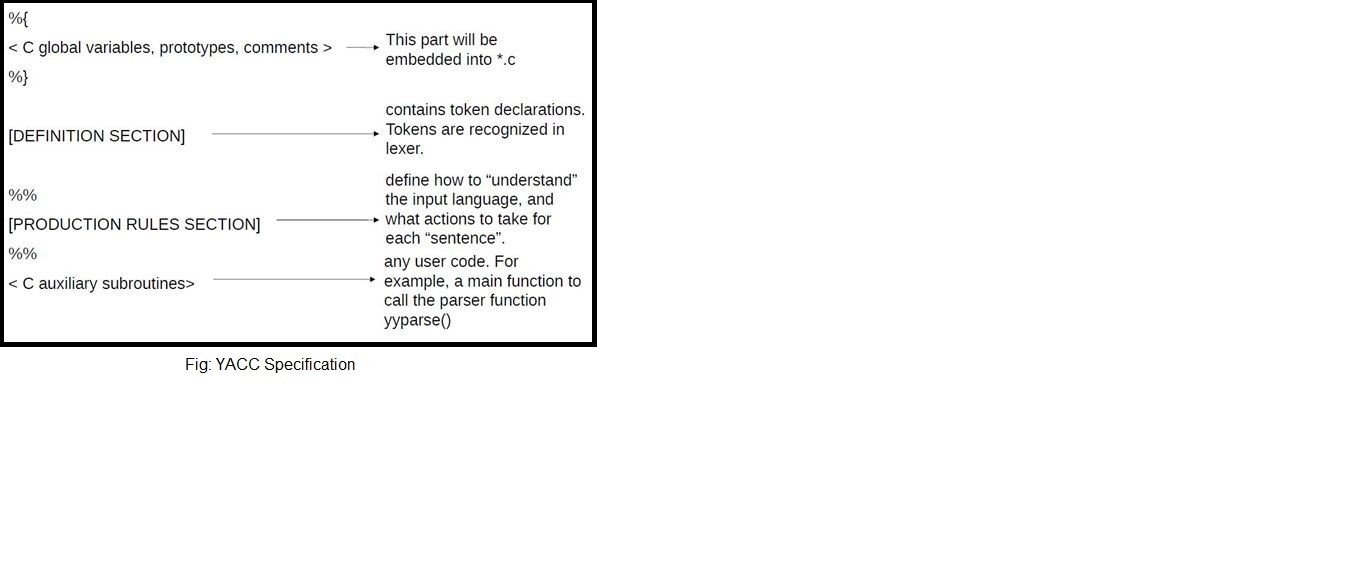
\includegraphics{yacc.png}
		
	\end{center}•
	\noindent
	YACC : What it is ?\\
	Yacc is a tool for automatically generating a parser given a grammar written in a yacc specification (.y file).\\
	
	\noindent
	Why Yacc?\\
	It is possible to create a simple parser using Lex alone. by making extensive use of the user-defined states (i.e start-conditions).\\ However, such a parser quickly becomes unmaintainable, as the number of user-defined states tends to explode.\\
	Once our input file syntax contains complex structures, such as “balanced” brackets, or contain s elements which are context-sensitive, we should be considering yacc.\\
	
	\noindent
	Precedence and Associativity:\\
	Bison allows you to specify operator precedence.
	\begin{enumerate}
		\item Left Associativity:\\
		The %left declaration makes all the opearotors left-associative.\\
		\item Right Associativity:\\
		The %right declaration makes all the opearotors right-associative.\\
		\item Non Associativity:\\
		The third alternative is %nonassoc,which declares that it is a syntax error to find the same operator twice“in a row”.\\
	\end{enumerate}•
	
	\noindent
	Simple Rule:\\
	Yacc rules define what is a legal sequence of tokens in our specification language. In our case, lets look at the rule for a simple expression form:\\
	$$E : E‘+’E$$
	$$| E‘-’E$$
	$$;$$
	This rule defines a non-terminal symbol,E in terms of the two tokens ‘+’ or ‘-’.\\
	In any case, yacc provides a formal method for dealing with the semanitic value of tokens. It begins with the lexer. Every time the lexer returns a value, it should also set the external variable yylval to the value of the token. Yacc will then retain the association between the token and the corresonding value of yylval.\\
	In order to accomodate a variety of different token-types, yylval is declared as a union of different types.\\
	
	\noindent
	Token Types:\\
	Token types are declared in yacc using the yacc declaration "\%union"\\
	
	\noindent
	\%union{\\
		int v; char s[10];\\
	}\\
	
	This defines yylval as being a union of the types (char) and (int). This is a classical C program union, so any number of types may be defined, and the union may even contain struct types, etc.\\
	We also need to tell yacc which type is associated with which token. This is done by modifying our \%token declarations to include a type, like this:\\
	
	\noindent
	\%token $<s>$ ID\\
	\%token $<v>$ NUM\\
	Yacc provides a simple yet elegant solution, by extending the concept of the “value” of a token to non-terminal symbols,like E.\\ First, we have to declare the E in our Yacc Declarations section, like this:\\
	
	\noindent
	\%type $<v>$ E\\
	
	\noindent
	Yacc Actions:\\
	Actions within yacc rules take the form:\\
	production : symbol1 symbol2 { action1 }\\
	| symbol3 symbol4 { action2 }\\
	;\\
	
	\noindent
	Using Token Types in Yacc Actions:\\
	Now that we have the token value, we want to make use of it. Yacc lets us refer to the value of a given token using a syntax similar to that of awk and perl. \$1 is the value of the 1st token, \$2 is the 2nd, and so on. Here is a typical example of an action:\\
	
	E : E‘+’E { \$\$=\$1$+$\$3; }\\
	| E$‘-’$E { \$\$=\$1-\$3; }\\
	;\\
	We assign the value of the left-hand-side of the rule by assigning a value to \$\$.\\
	
	\noindent
	The storage space for our \$\$ is just another value attached to a token, and this is handled automatically by yacc. So no crash. And we’ve removed the unwanted duplication of code in our actions.\\
	
	\noindent
	The Yacc Default Action\\
	In the absence of explicit action, yacc applies a default action of:\\
	{ \$\$$=$\$1; }\\
	Or, put simply, the left-hand-side inherets the value from the 1st symbol on the right-hand-side.\\
	
	\noindent
	Built in Functions:\\
	\begin{enumerate}
		\item yyparse():\\
		Yacc generates a single function called yyparse(). This function requires no parameters. and returns either a 0 on success, and 1 on failure. “Failure” in the case of the parser means “if it encounters a syntax error”.\\
		\item yyerror():\\
		The yyerror() function is called when yacc encounters an invalid syntax. The yyerror() is passed a single string (char*) argument.This string usually just says “parse error”, so on its own.\\
		Syntax of basic yyerror() function like this:\\
		yyerror(char *err)\\
		{ fprintf(stderr, “\%s”,err);\\
		}
	\end{enumerate}•
	
	\noindent
	Debugging the Prototype\\
	Sometimes YACC may generate a couple of messages/warnings.Both of these warnings mean that there is an ambiguity in our ruleset.\\
	A Shift operation is what the parser does when it saves a token for later use. (Actually, it pushes the token onto a stack).\\
	A Reduce operation is what the parser does when resolves a set of tokens into a single, complete rule.\\
	
	\noindent
	Types of Conflicts:\\
	\begin{enumerate}
		\item Shift/Reduce Conflicts :\\
		shift/reduce conflict occurs when there would be enough tokensshifted (saved) to make up a complete rule, but the next token may allow a longer rule to be applied. In the event of a shift/reduce conflict, the parser will opt for the shift operation, and hence try to build the longer rule. If your grammar has “optional” structures, such as an optional “else” following an “if” statement, then it may not be possible to eliminate all shift/reduce conflicts from the grammar rules.\\
		\item Reduce/Reduce Conflicts :\\
		reduce/reduce conflict occurs when the same set of tokens can beused to form two different rules. In the event of a reduce/reduce conflict, the parser will use the first rule that appears in the grammar. You can think of this as being analogous to lex’s “first match” rule. Reduce/reduce conflicts are usually an indication of an error in the way the grammar rules have been defined, as the whole point of having a grammar is to avoid such blatant ambiguities. It is usually possible (and desirable) to eliminate all reduce/reduce conflicts from your grammar rules, either by rewriting some rules, or redefining the grammar (if possible).
		
	\end{enumerate}•
	
	\noindent
	Resolving Shift/Reduce and Reduce/Reduce Conflicts:\\
	
	In order to find out which rules are affected by these conflicts, you will need to refer to the *.output file generated by running yacc with the $-$v flag, for example: bison $-$v olmenu-proto1.y This will generate the usual *.tab.c file, plus an additional LALR.output file. This file will tell you which rules are causing the conflicts mentioned.\\
	Note that there are some incompatibilities at this level between yacc and bison. Yacc likes to call its output files y.tab.c for the parser and y.tab.h for the token definitions. Bison prefers to use basename.tab.c and basename.tab.h (respectively). Bison will generate y.tab.c and y.tab.h if it is invoked with the $-$y flag.\\
	
	\noindent
	LALR Parser(Lookahead-LR Parser) :\\
	Generally, the LALR parser refers to the LALR(1) parser.The “(1)”denotes one-token lookahead, to resolve differences between rule patterns during parsing. The LALR parser is based on the LR(0) parser, so it can also be denoted LALR(1)$ =$ LA(1)LR(0) (1 token of lookahead, LR(0)) or more generally LALR(k) $= $LA(k)LR(0) (k tokens of lookahead, LR(0)).\\
	
	LALR parsers offer many of the advantages of SLR and Canonical-LR parsers, by combining the states that have the same kernels (sets of items, ignoring the associated lookahead sets). Thus, the number of states is the same as that of the SLR parser, but some parsing-action conflicts present in the SLR parser may be removed in the LALR parser. LALR parsers have become the method of choice in practice.\\
	
	\noindent
	Construction of LALR Parsing Table :\\
	\begin{enumerate}
		\item Obtain the canonical collection of sets of LR(1) items.
		\item If more than one set of LR(1) item exists in the canonical collectionobtained that have identical cores or LR(0)s,but which have different lookaheads then combine these sets of LR(1) items to obtain a reduced collection or of sets of LR(1) items.
		\item Construct the parsing table by using this reduced collection as follows: for action table:
		\begin{enumerate}
			\item For each state Ii in C1 do for every terminal symbol a do ifgoto(Ii,a)$=$Ij then make action [Ii,a]$=$Sj //for shift
			\item For every state Ii in C1 whose underlying sets of items containsan items of the form A-> alpha., a do make action[Ii,a]$=$Rr
			\item Make [Ii,\$]$=$accept if ii contains an item S1->S.,\$. For goto table:\\
			For every Ii in C1 do For every nonterminal A do if goto(Ii,A)=Ij then make goto (Ii,A)=Ij.
		\end{enumerate}•
	\end{enumerate}•
	
	
	Example:\\
	Consider the following augmented grammer.\\
	S’$->$ S\\
	S $->$CC\\
	C $->$ cC | d\\
	
	Solution:\\
	We begin with computing closure-set{}.\\
	Io: S$->.$S, \$ S$->.$CC, \$\\
	C$->.$cC, c/d\\
	C$->.$d, c/d\\
	I1: S’$->$ S.,\$\\
	I2: S$->$C.C,\$\\
	C$->.$cC, \$\\
	C-$>.$d, \$\\
	I3: C$->$c.C, c/d\\
	C$->.$cC, c/d\\
	C$->.$d, c/d\\
	I4: C$->$ d., c/d\\
	I5: S$->$ CC., \$\\
	I6: C$->$c.C,\$\\
	C$->.$cC,\$\\
	C$->.$d, \$\\
	I7: C$->$ d., \$\\
	I8: C$->$ cC., c/d\\
	I9: C$->$cC., \$\\
	There are three pairs of sets of items that can be merged.I3 and I6 are replaced by their union:\\
	I36: C$->$c.C, c/d/\$\\
	C$->.$cC, c/d/\$\\
	C$->$.d, c/d/\$\\
	I4 and I7 are replaced by their union: I47: C $->$d., c/d/\$\\
	and I8 and I9 are replaced by their union: I89: C $->$cC., c/d/\$\\
	
	\noindent
	LALR parsing table for the above grammer can be constructed as follows:\\
	\begin{center}
		\begin{tabular}{|c|c|c|c|c|c|}
			•$$ & $c$ & $d$ & $\$$ & $S$ & $C$ \\ \hline
			•$0$ & $s36$ & $s47$ & & $1$ & $2$ \\ \hline
			•$1$ & & & $Accept$ & &\\ \hline
			•$2$ & $s36$ & $s47$ & & &$5$ \\ \hline
			•$36$ & $s36$ & $s47$ & & &$89$ \\ \hline
			•$47$ & $r3$ & $r3$ & $r3$& & \\ \hline
			•$5$ &  &  &$r1$ & & \\ \hline
			•$89$ & $r2$ & $r2$ & $r2$& & \\ \hline
			\end{tabular}•
			\end{center}•
			
			\noindent
			Advantage :\\
			LALR parser is quite efficient at finding the single correct bottom-up parse in a single left-to-right scan over the input stream, because it does not need to use backtracking\\
			
			\noindent
			Command:\\
			\$ lex $<program name>.$l\\
			\$ yacc -d $<$program name$>.$y\\
			\$ gcc lex.yy.c y.tab.c -ll -ly\\
			\$ ./a.out\\
			
			\noindent
			Conclusion:\\
			Thus, we have constructed LALR Parser to evaluate given expression using Lex and Yacc.
			
			\begin{center}
			\begin{tabular}{|c|c|c|c|c|}
			•$Roll$ $No$ & $Name$ $of$ $Student$ & $Date$ $of$ $performance$ & $Date$ $of$ $Checking$ & $Signature$ $of$ $Staff$ \\ \hline
			\documentclass[11pt]{article}
			\usepackage{graphicx}
			
			\begin{document}
			
			\begin{center}
			Assignment No 2
			\end{center}•
			
			\noindent
			Aim:\\Implement Recursive Descent Parser for some language.\\
			
			\noindent
			Software:\\
			\begin{enumerate}
			\item Linux Operating System
			\item GCCcompiler
			\end{enumerate}•
			
			\noindent
			MATHEMATICALMODEL:\\
			
			\noindent
			S={s,e,i,o,f,DD,NDD,success,failure}\\
			s=Start of program\\
			e=The end of program\\
			i=Input String to be parsed. o=Output of the parser, ie, \\
			ValidString(if given input string is valid) OR Parse error (if given input string is invalid)\\
			Success-Parser gives expected output\\
			Failure-Power Failure, Insufficient Memory. f={E, Eprime, T, Tprime, F}\\
			
			\noindent
			Theory:
			
			\noindent
			Recursive Descent Parser\\
			
			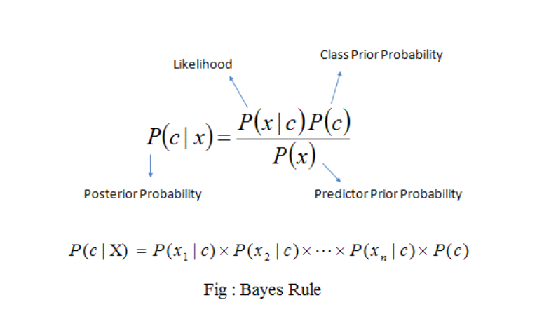
\includegraphics{image1.png}
			
			\noindent
			This is a top-down parser in which the parser attempts to verify that the syntax of the input stream is correct as it is read from left to right. A basic operation necessary for this  involves reading characters from the input stream and matching then with terminals from the grammar that describes the syntax of the input.RDP will look ahead one character and advance the input stream reading pointer when proper matches occur.\\
			
			RDP consists of a set of procedures, one for each non terminal. Execution begins with the procedure of the start symbol, which halts and announces success if its procedure body scans the entire input string (valid).\\
			
			RDP may require back tracking; that is, it may require repeated scans over the input. Parse tree with all possible alternatives. If one alternative doesn’t workout, backtrack and use another alternative. If even after using allalternatives, required string is not formed, string is invalid.Consider the following grammar.The required string is ”cad”:\\
			
			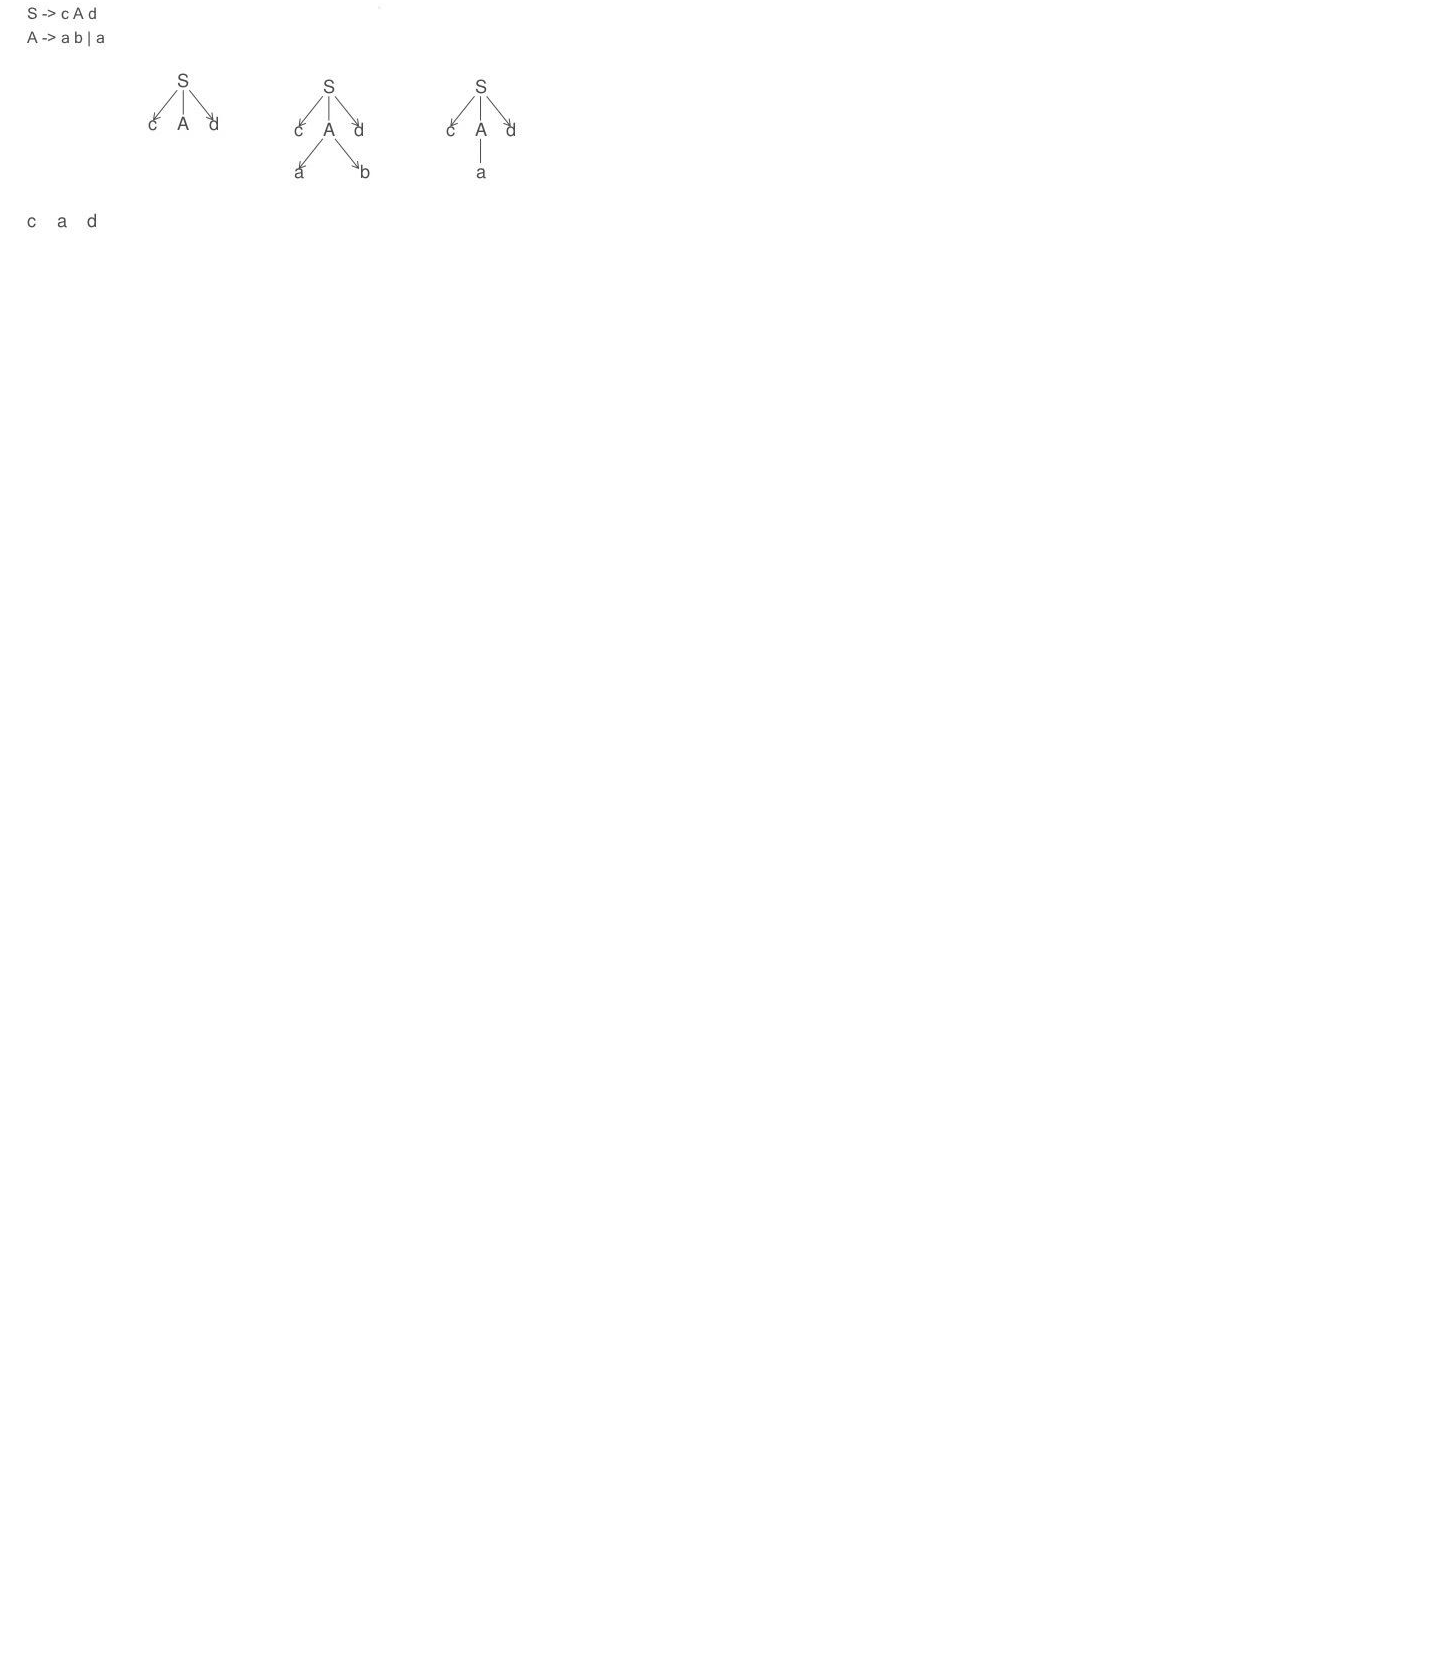
\includegraphics{image2.png}
			
			\noindent
			Advantage:\\
			1.Construction of RDP is easy.\\
			
			\noindent
			Disadvantages:\\
			1.Backtracking(Not allowed in many programming languages)\\
			2.For left recursive grammar RDP parser may fall in infinite loop.\\
			3.Large space to be traversed (multi level backtracking as parse tree is derived blindly)\\
			
			\noindent
			Construction of Recursive Descent Parser:\\
			\begin{enumerate}
			\item If input symbol is non terminal then a call to the procedure correspond-ing to the non terminal is made.
			\item If input symbol is terminal then it is matched with the look ahead from input. The look ahead pointer has to be advanced on matching of the input symbol.
			\item If the production rule has many alternates then all these alternates has to be combined into a single body of procedure.
			\item The parser should be activated by a procedure corresponding to the start symbol.
			
			\end{enumerate}•
			
			\noindent
			Command:\\
			\$gccRDescent.c\\
			\$./a.out\\
			
			\noindent
			CONCLUSION:\\
			Thus we have constructed Recursive Descent Parser for given grammar.\\
			
			\begin{center}
			\begin{tabular}{|c|c|c|c|c|}
			•$Roll$ $No$ & $Name$ $of$ $Student$ & $Date$ $of$ $performance$ & $Date$ $of$ $Checking$ & $Signature$ $of$ $Staff$ \\ \hline
			•$BECOC357$ & Sunny Shah& 21 / 07 / 2017& 23 / 08 / 2017 &  \\ \hline
			\end{tabular}•
			\end{center}•
			
			\newpage
			\section{PLAGARISM REPORT :}
			\begin{figure}[h!]
			\centering
			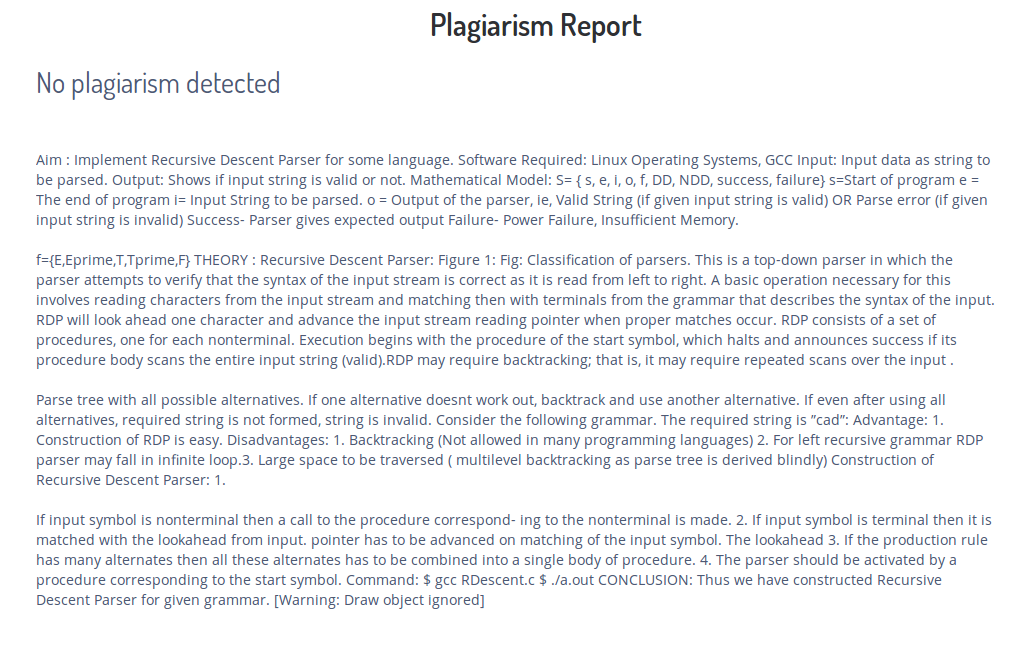
\includegraphics[height=4in,width=4in]{plagiarism2.png}
			\caption{Plagarism Checker www.smallseotools.com/plagarism-checker}
			\end{figure}
			\newpage
			\end{document}
			
			
			\end{tabular}•
			\end{center}•
			\newpage
			\section{PLAGARISM REPORT :}
			\begin{figure}[h!]
			\centering
			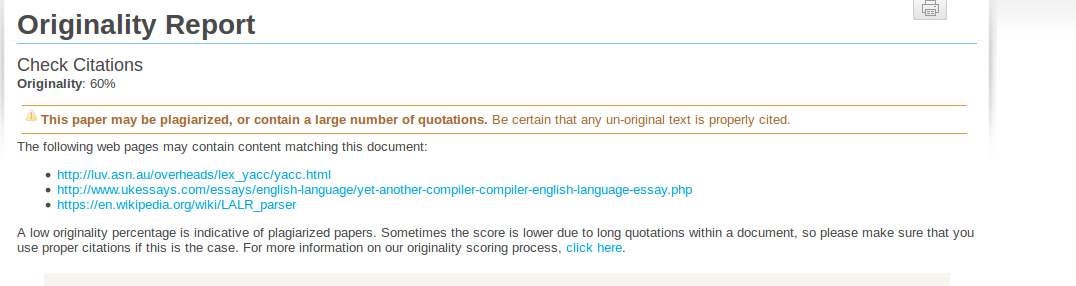
\includegraphics[height=5in,width=6in]{plagiarism3.png}
			\caption{Plagarism Checker www.smallseotools.com/plagarism-checker}
			\end{figure}
			\newpage
			\end{document}